\documentclass[11pt,a4paper]{article}
\usepackage[a4paper,hmargin=1in,vmargin=1in]{geometry}
\usepackage{pgfplots}
\pgfplotsset{compat=1.17}

\usepackage[czech]{babel}
\usepackage[utf8]{inputenc}
\usepackage[T1]{fontenc}

\usepackage[nodayofweek]{datetime}
\newdate{date}{17}{6}{2023}

\usepackage{stddoc}
\usepackage{lipsum}
\usepackage{subcaption}
% \usepackage[square,numbers]{natbib}
% \usepackage[nottoc]{tocbibind}

\newcommand{\plus}{{\texttt{+}}}
\renewcommand{\Re}{\operatorname{Re}}
\renewcommand{\Im}{\operatorname{Im}}
\newcommand{\fourier}[3]{\mathcal{F}_{#1}\!\left[#2\right]\!\left(#3\right)}
\newcommand{\ifourier}[3]{\mathcal{F}^{-1}_{#1}\!\left[#2\right]\!\left(#3\right)}
\newcommand{\Ohm}{\mathrm{\Omega}}
\newcommand{\kOhm}{\mathrm{k\Omega}}
\newcommand{\dB}{\mathrm{dB}}
\newcommand{\dBm}{\mathrm{dBm}}
\newcommand{\MHz}{\mathrm{MHz}}
\newcommand{\GHz}{\mathrm{GHz}}
\newcommand{\kHz}{\mathrm{kHz}}


\begin{document}

\pagenumbering{arabic}

% Header
\begin{center}
    {\LARGE\textbf{Laboratorní úloha č. 12}}\\[3mm]
    \begin{minipage}{0.4\textwidth}
        \begin{flushleft}
            \textsc{\displaydate{date}}
        \end{flushleft}
    \end{minipage}
    ~
    \begin{minipage}{0.4\textwidth}
        \begin{flushright}
            \textsc{Martin Šimák}
        \end{flushright}
    \end{minipage}
    \noindent\rule{14.5cm}{0.4pt}
\end{center}

\paragraph*{Měření SMD komponent} Laboratorní úloha ukazuje využití vektorového měření pro určování parametrů SMD komponent s referenční rovinou měření přímo na okrajích pouzdra.

\subsection*{Úkoly měření}
\begin{enumerate}
    \item Měření kondenzátorů $10\ \mathrm{pF}$ od ATC a Johanson Technology.
    \item Měření induktorů $3.3\ \mathrm{nH}$ a $27\ \mathrm{nH}$ od Johanson Technology.
    \item Určení parametrů náhradního modelu rezistoru v pouzdru 0402.
\end{enumerate}

\subsection*{Použité přístroje a komponenty}
\begin{itemize}
    \item Vektorový analyzátor R\&S ZVA67 (10~MHz až 67~GHz)
    \item Kalibrační sada vyrobena na substrátu Rogers CuClad 233 tl. $0.254\ \mathrm{mm}$
\end{itemize}

\subsection*{Popis měření}

% Task 1
\paragraph*{Kalibrace vektorového analyzátoru} Úkolem měření je zjistit S-parametry SMD komponent. Pro měření s referenční rovinou přímo na okrajích jejich pouzdra je potřeba zkalibrovat na plošném spoji. Taková kalibrace se dá provést pomocí správně navržené kalibrační sady, která bude vyrobena na stejném substrátu jako vedení, kde chceme SMD komponenty následně použít. Na nízkých frekvencích do několika GHz se dá využít kalibrační metoda TRM (\emph{thru}, \emph{reflect}, \emph{match}) a na vyšších frekvencích pak TRL (\emph{thru}, \emph{reflect}, \emph{line}).
\begin{figure}[!ht]
    \centering
    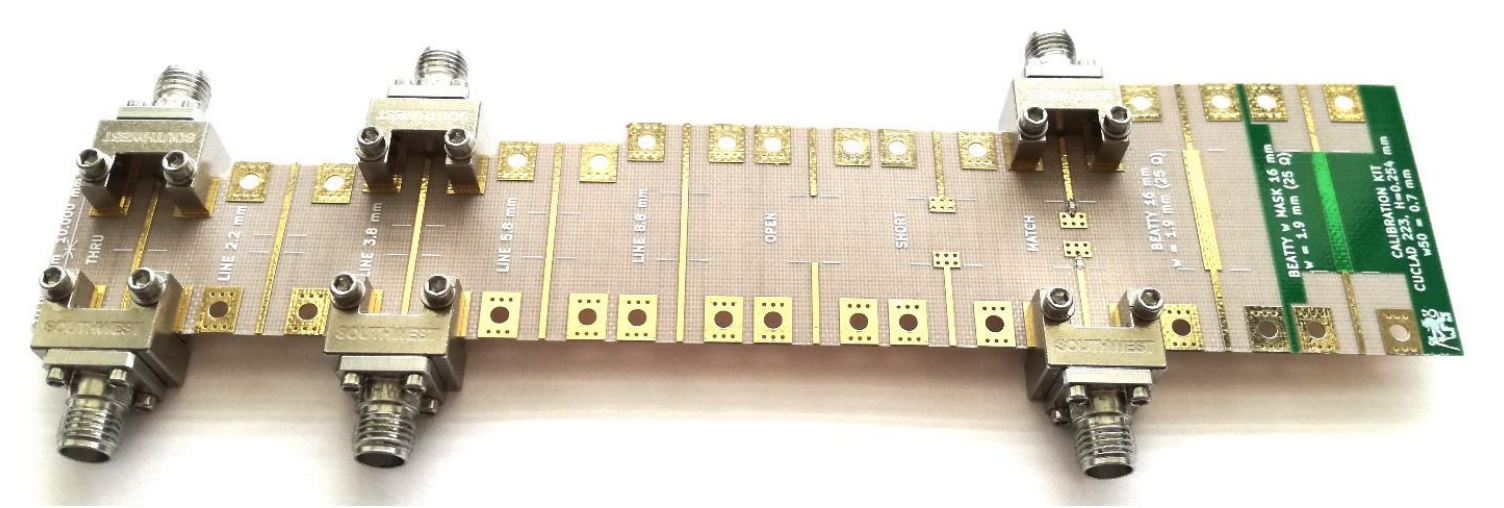
\includegraphics[width=.7\textwidth]{src/kalibracni-sada.png}
    \caption{\label{fig:kalibracni-sada}Kalibrační sada na substrátu Rogers CuClad 233}
\end{figure}

Kalibrační sada je zobrazena na obrázku~\ref{fig:kalibracni-sada}. Obsahuje několik kalibračních standardů, ke kterým je možné se připojit pomocí SuperSMA \href{https://mpd.southwestmicrowave.com/product-category/end-launch-connectors/}{End-Launch} konektorů od Southwest Microwave typu 292-04A-5. Tyto konektory pracují do 27~GHz a poskytují přijatelnou opakovatelnost montáže. Referenční rovina kalibračních standardů je 10~mm od okraje plošného spoje, tj. uprostřed standardu thru. Na substrátu má $50\Ohm$ mikropáskové vedení šířku 0.7~mm a efektivní permitivitu asi 1.95. Tyto údaje lze použit k definici kalibrační sady ve vektorovém analyzátoru.

Kalibrační metoda TRL je ze své podstaty úzkopásmová a je nejpřesnější pouze na těch frekvencích, kdy je mezi přenosy na vedeních představujících kalibry thru a line fázový rozdíl $\pi/2$, tedy $\lambda/4$. K tomu dochází jen v daných frekvenčních bodech a v okolním pásmu se již měří méně přesně. Na frekvencích, kde je mezi vedeními thru a line fázový rozdíl 0, selhává kalibrace docela. Pro pokrytí širšího frekvenčního pásma se tedy používá více kalibračních standardů line, které musí mít vhodnou fyzickou délku. Na nízkých frekvencích by délka kalibru line vycházela neprakticky dlouhá a dá se tedy nahradit kalibrem match.
\begin{figure}[!ht]
    \centering
    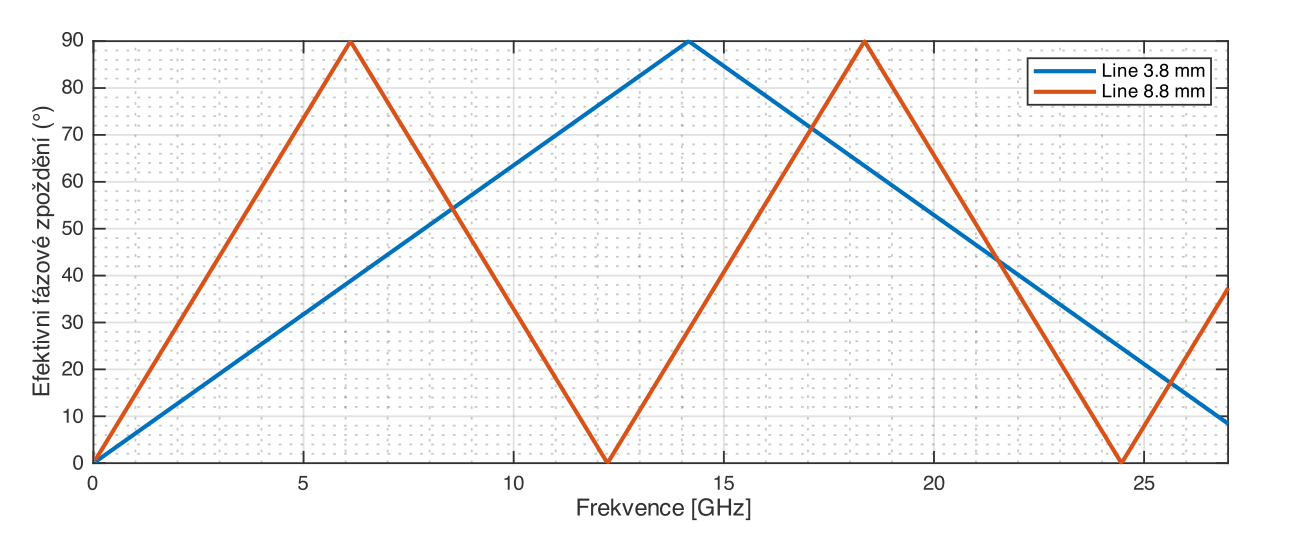
\includegraphics[width=.8\textwidth]{src/fazove-zpozdeni.png}
    \caption{\label{fig:fazove-zpozdeni}Efektivní fázové zpoždění použitých standardů line}
\end{figure}

Vektorový analyzátor uvedeme do základního nastavení a nastavíme frekvenční pásmo na 50~MHz až 27~GHz s krokem 50~MHz a výkonem 0~dBm. Dále ve dvou grafech zobrazíme měření přenosu a odrazu a provedeme TRL kalibraci VNA pomocí kalibrační sady. Měříme kalibrační standardy požadované VNA firmwarem, ale line měříme pouze s délkami 3.8~mm a 8.8~mm. Jejich efektivní fázový rozdíl oproti kalibru thru je zobrazen na obrázku~\ref{fig:fazove-zpozdeni}. V okolí pásma 6~GHz se na kalibraci podílí delší line, kdežto v okolí 14~GHz až do nejvyšší frekvence ta kratší. Ve VNA je použita základní, tzv. \emph{přepínaná}, metoda TRL, která na základě pravidel určených výrobcem rozhodne, pro které pásmo použije jaký kalibr line. Zároveň na nejnižších frekvencích použije kalibr match, ale do jaké frekvence ho použije opět záleží na konkrétní implementaci metody. Kalibrační metoda TRM je jen speciální případ metody TRL.

Pro verifikaci kalibrace využijeme tzv. Beatty line, což je typicky $25\Ohm$ nebo $100\Ohm$ úsek vedení se známou délkou mezi referenčními rovinami měření. Tento obvod tvoří rezonátor, jehož přenos a odrazy jsou analyticky vypočitatelné při zanedbání diskontinuit na okrajích rezonátoru. Měření Beatty line můžeme porovnat s načteným Touchstone souborem tohoto standardu vypočteného v AWR (nastavení \emph{File/Trace Data/Import Complex Data...}). Simulační schéma je na obrázku~\ref{fig:beatty-line-awr} a porovnání naměřených dat s S-parametry simulovaného obvodu je možné učinit z grafů na obrázku~\ref{fig:beatty-line}.
\begin{figure}[!ht]
    \centering
    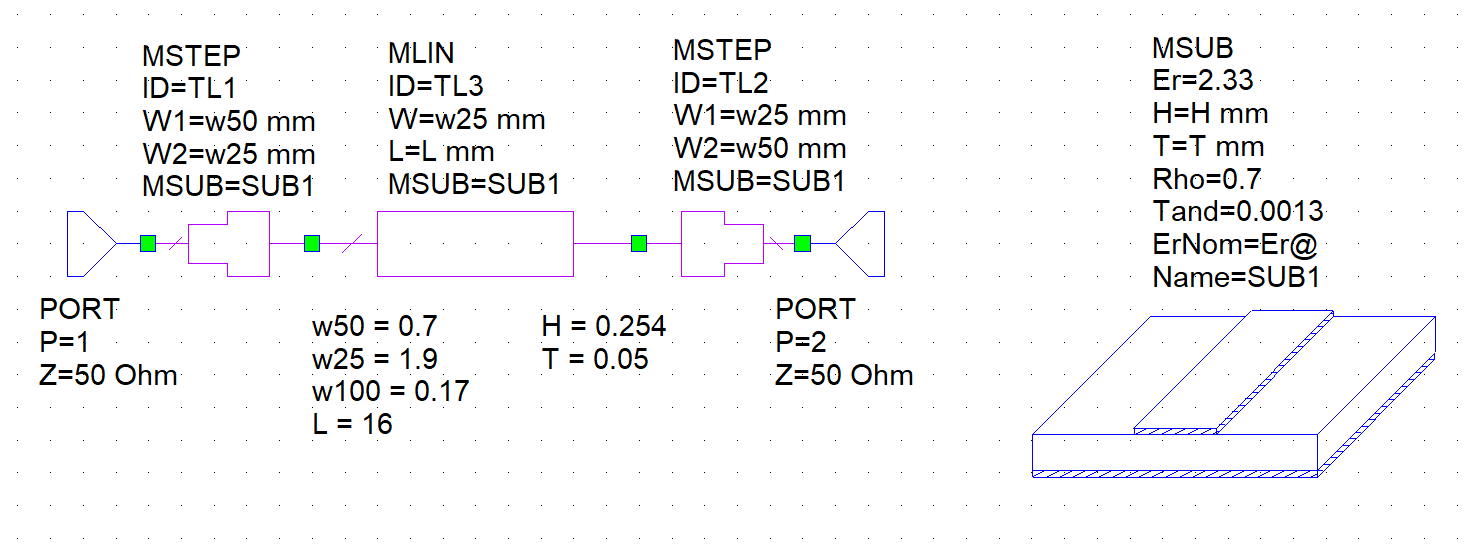
\includegraphics[width=.8\textwidth]{src/beatty-line-awr.png}
    \caption{\label{fig:beatty-line-awr}Simulační model verifikační Beatty line v AWR}
\end{figure}
\begin{figure}[!ht]
    \centering
    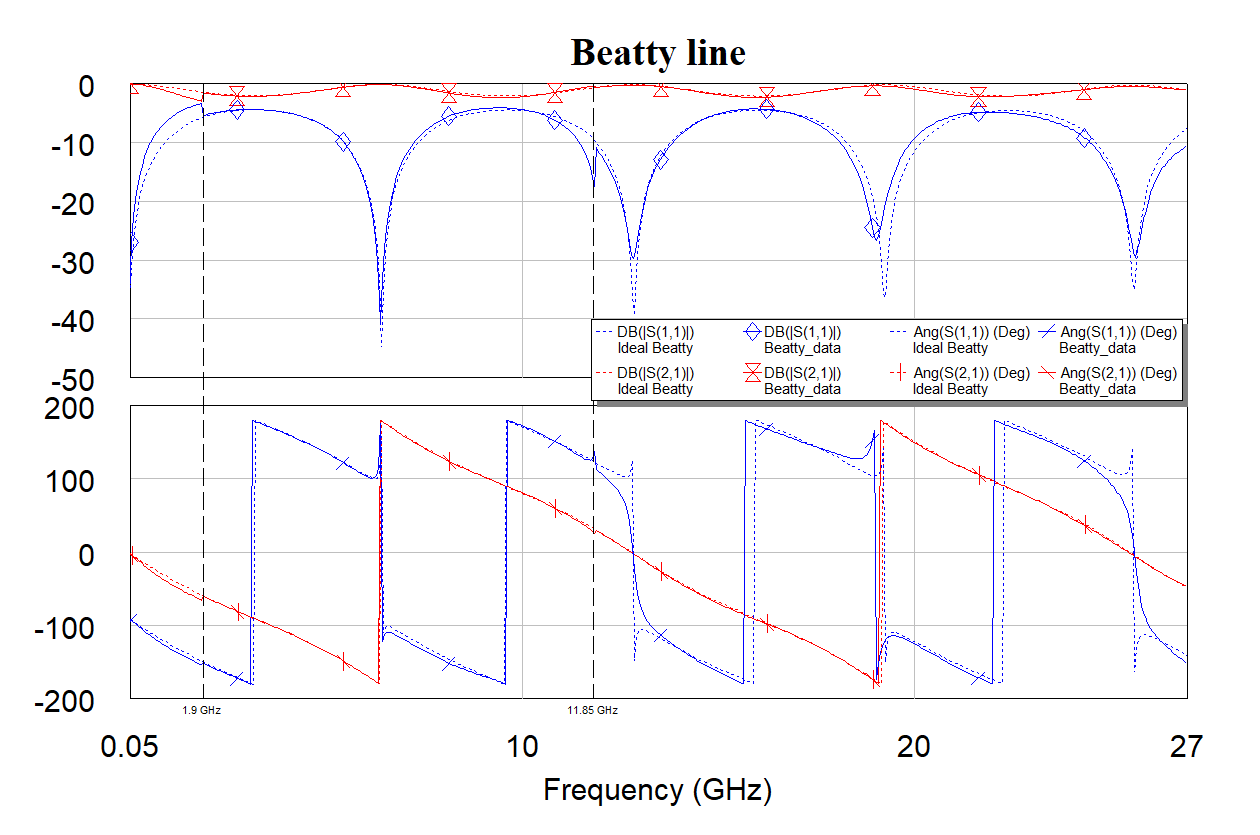
\includegraphics[width=.9\textwidth]{src/beatty-line.png}
    \caption{\label{fig:beatty-line}Porovnání naměřených S-parametrů Beatty line se simulačním modelem}
\end{figure}
\subparagraph*{Úkol} \emph{Diskutujte rozdíly mezi měřením a simulací.} Jak je vidět z obrázku~\ref{fig:beatty-line}, kalibrace byla provedena s přijatelnou přesností. Experimentální data dobře sedí na S-parametry simlovaného obvodu, zejména na nižších frekvencích, kde byla kalibrace provedena metodou TRM. Jediné značnější deviace od simulace jsme naměřili diskrétně na frekvencích $~1.9\ \GHz$ a $~11.85\ \GHz$, kde očividně dochází během přepínané kalibrace ke změně kalibru: první přechod je zřejmě z delší line na kratší a druhý z kratší line na match.%
    \footnote{Kalibr match je totiž ekvivalentem nekonečně dlouhého přizpůsobeného vedení.}
Lze usoudit, že vyšší přesnosti bychom v tomto scénáři dosáhli jedině dokonalejší kalibrační metodou nebo použitím více kalibrů line o různých (vhodně zvolených) délkách.

% Task 2
\paragraph*{Měření kondenzátorů} Kondenzátor od ATC (\href{https://rfs.kyocera-avx.com/millimeter-wave-surface-mount-capacitors}{datasheet}) je v pouzdru velikosti 0603 (zhruba $1.5 \times 0.8\ \mathrm{mm}$), zatímco kondenzátor od Johanson Technology (\href{https://www.johansontechnology.com/r07s}{datasheet}) je v pouzdru velikosti 0402 (zhruba $1 \times 0.5\ \mathrm{mm}$). S-parametry obou kondenzátorů dodané výrobcem jsou dostupné pro simulace v knihovnách softwaru AWR.

Naměřené S-parametry kondenzátorů jsou spolu s daty od výrobce zakresleny do polárního diagramu v obrázku~\ref{fig:capacitors}. Z přímého porovnání je zřejmé, že oba kondenzátory sledují velice podobný průběh pro data experimentální i dodaná výrobcem. Nejmarkantnější deviaci lze pozorovat ve fázovém posunu, který je nejspíše způsoben tím, že data od výrobce jsou udána pro referenční rovinu uprostřed pouzdra, kdežto my jsme data měřili s referenční rovinou na okrajích.
\begin{figure}[!ht]
    \centering
\begin{subfigure}{0.45\textwidth}
    \centering
    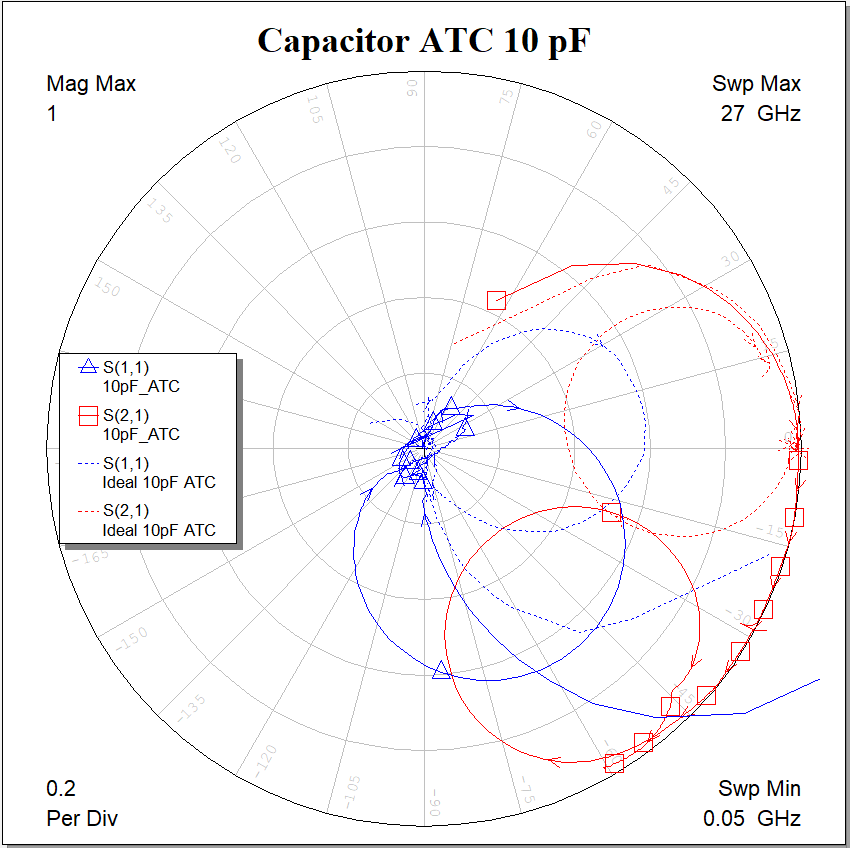
\includegraphics[width=\textwidth]{src/capacitor-10pF-ATC.png}
    \caption{$10\ \mathrm{pF}$ ATC}
\end{subfigure}
\begin{subfigure}{0.45\textwidth}
    \centering
    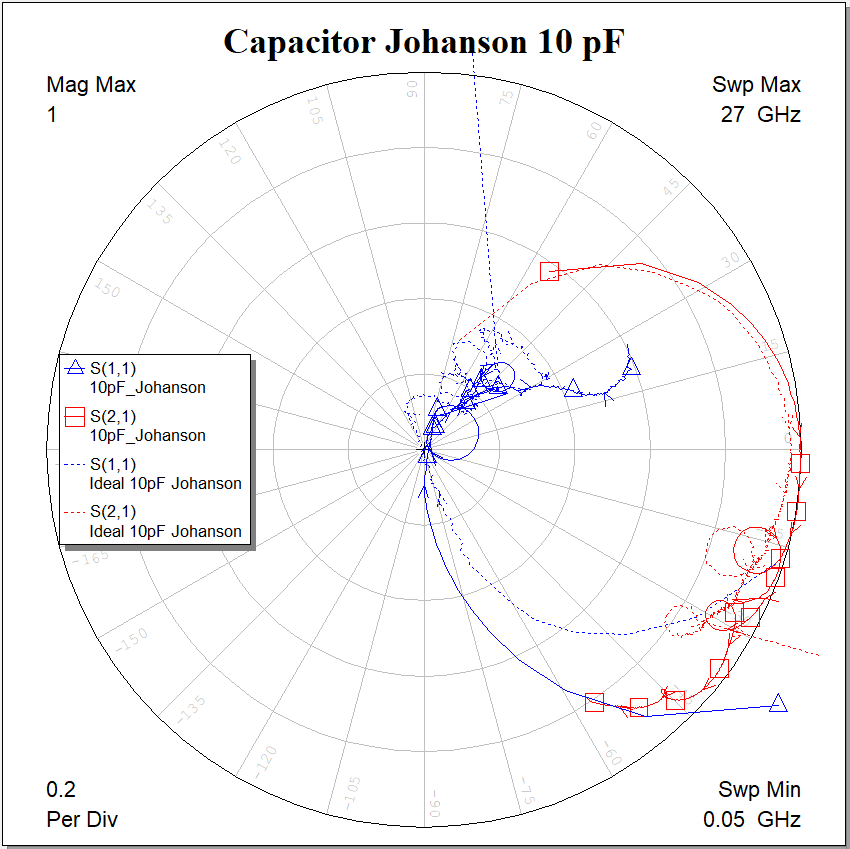
\includegraphics[width=\textwidth]{src/capacitor-10pF-Johanson.png}
    \caption{$10\ \mathrm{pF}$ Johanson Technology}
\end{subfigure}
\caption{\label{fig:capacitors}Porovnání naměřených S-parametrů kondenzátorů s daty dodanými výrobcem}
\end{figure}

% Task 3
\paragraph*{Měření induktorů} Oba induktory jsou od společnosti Johanson Technology a patří do řady \emph{RF Wirewound Chip Inductor} (\href{https://www.johansontechnology.com/wirewound-inductors}{datasheet}). Induktor s hodnotou $3.3\ \mathrm{nH}$ je v pouzdru 0402, zatímco $27\mathrm{nH}$ induktor je v pouzdru 0603. S-parametry obou induktorů dodané výrobcem jsou dostupné pro simulace v knihovnách softwaru AWR.

Naměřené S-parametry induktorů jsou spolu s daty od výrobce zakresleny do polárního diagramu v obrázku~\ref{fig:inductors}. Induktor s hodnotou $3.3\ \mathrm{nH}$ v pouzdru 402 má hladší frekvenční průběh a dobře sedí na data od výrobce přibližně až do 20~GHz. U Induktoru s hodnotou $27\ \mathrm{nH}$ je podobnost mezi naměřenými S-parametry a daty od výrobce výrazně horší. Data se jeví fázově posunuta a značně dříve od sebe divergují (zhruba od 16~GHz). Po celý frekvenční průběh se nezanedbatelně liší amplituda i fáze.
\begin{figure}[!ht]
    \centering
\begin{subfigure}{0.45\textwidth}
    \centering
    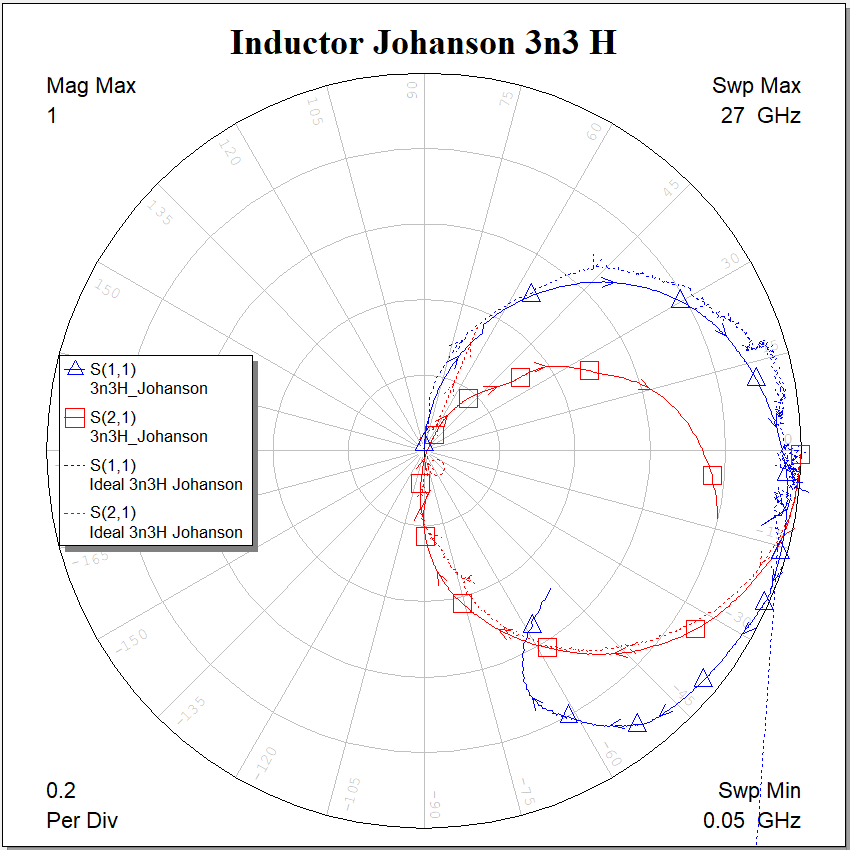
\includegraphics[width=\textwidth]{src/inductor-3n3H-Johanson.png}
    \caption{$3.3\ \mathrm{nH}$ Johanson Technology}
\end{subfigure}
\begin{subfigure}{0.45\textwidth}
    \centering
    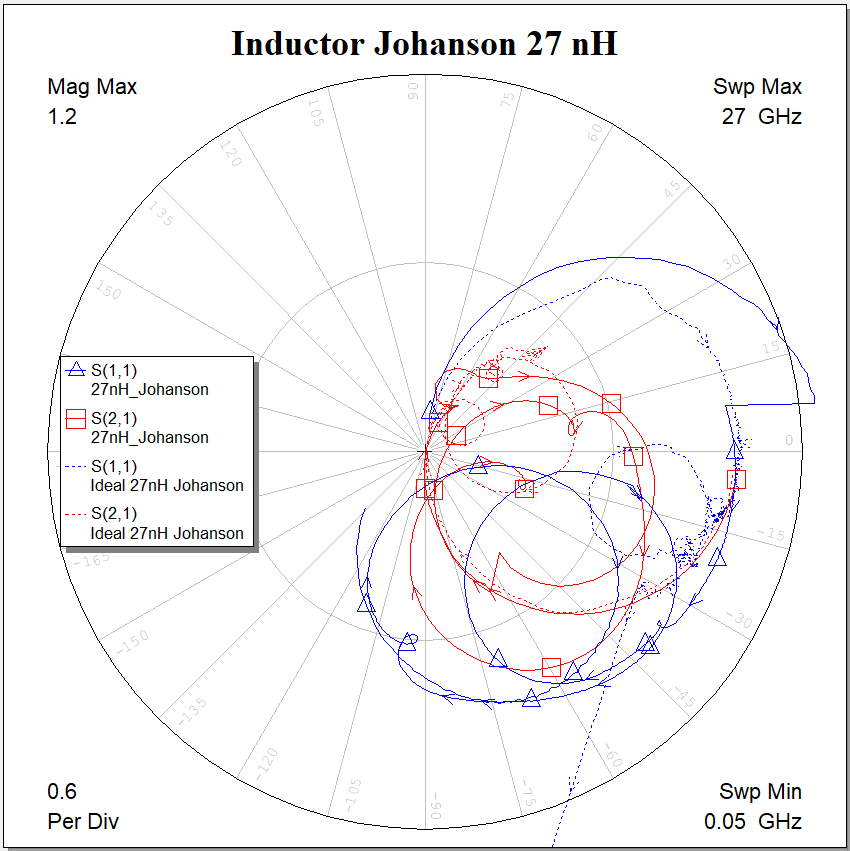
\includegraphics[width=\textwidth]{src/inductor-27nH-Johanson.png}
    \caption{$27\ \mathrm{nH}$ Johanson Technology}
\end{subfigure}
\caption{\label{fig:inductors}Porovnání naměřených S-parametrů induktorů s daty dodanými výrobcem}
\end{figure}

% Task 4
\paragraph*{Určení parametrů náhradního modelu rezistoru} Předmětem následující části měření jsou rezistory s hodnotami $2.2\ \Ohm$, $51\ \Ohm$ a $100\ \kOhm$, všechny tři v pouzdru 0402. Tato tři měření dále využíváme pro odhad parametrů náhradního obvodového modelu pouzdra, který je zobrazen na obrázku~\ref{fig:nahradni-model-pouzdra} pro rezistor s hodnotou $2.2\ \Ohm$.
\begin{figure}[!ht]
    \centering
    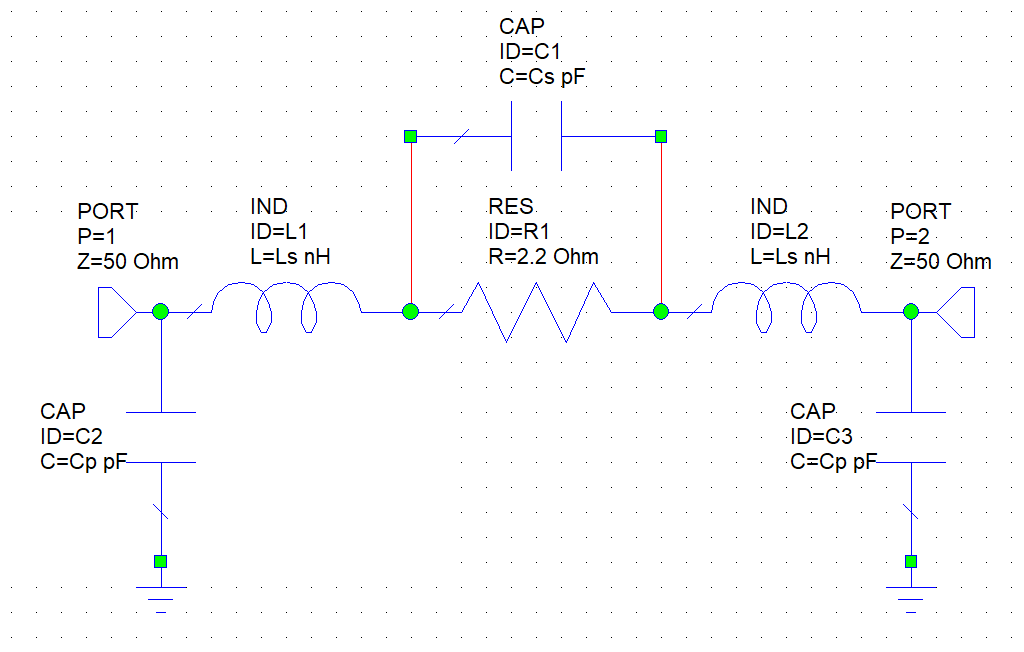
\includegraphics[width=.6\textwidth]{src/nahradni-model-pouzdra.png}
    \caption{\label{fig:nahradni-model-pouzdra}Náhradní model $2.2\Ohm$ rezistoru v pouzdru}
\end{figure}

Manuálním laděním hodnot sériové capatiy $C_s$, paralelních kapacit $C_p$ a sériových indukčností~$L_s$ z obrázku~\ref{fig:nahradni-model-pouzdra} lze iterativně dojít k hodnotám, za nichž zhruba odpovídají všechny tři frekvenční průběhy naměřených S-parametrů se simulovanými daty. Výsledek tohoto snažení je vidět na obrázku~\ref{fig:resistors} a takto zjištěné hodnoty parametrů pouzdra 0402 jsou zaneseny v tabulce~\ref{table:parametry-pouzdra}.
\begin{figure}[!ht]
    \centering
\begin{subfigure}{0.45\textwidth}
    \centering
    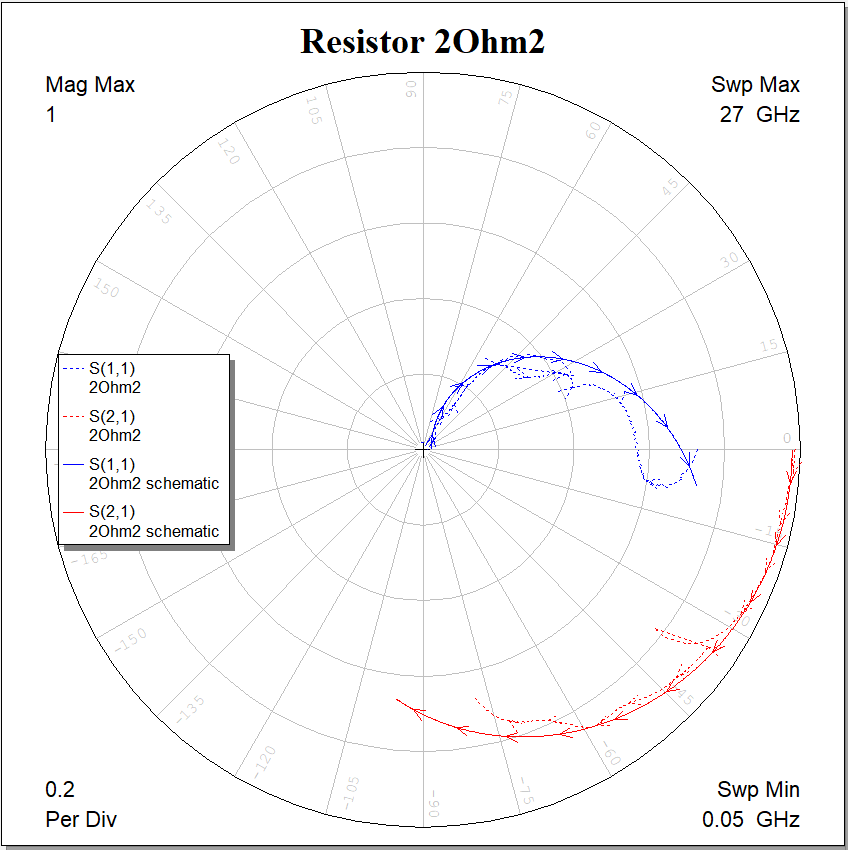
\includegraphics[width=\textwidth]{src/resistor-2Ohm2.png}
    \caption{\label{fig:resistor-2Ohm2}$2.2\Ohm$ rezistor}
\end{subfigure}
\begin{subfigure}{0.45\textwidth}
    \centering
    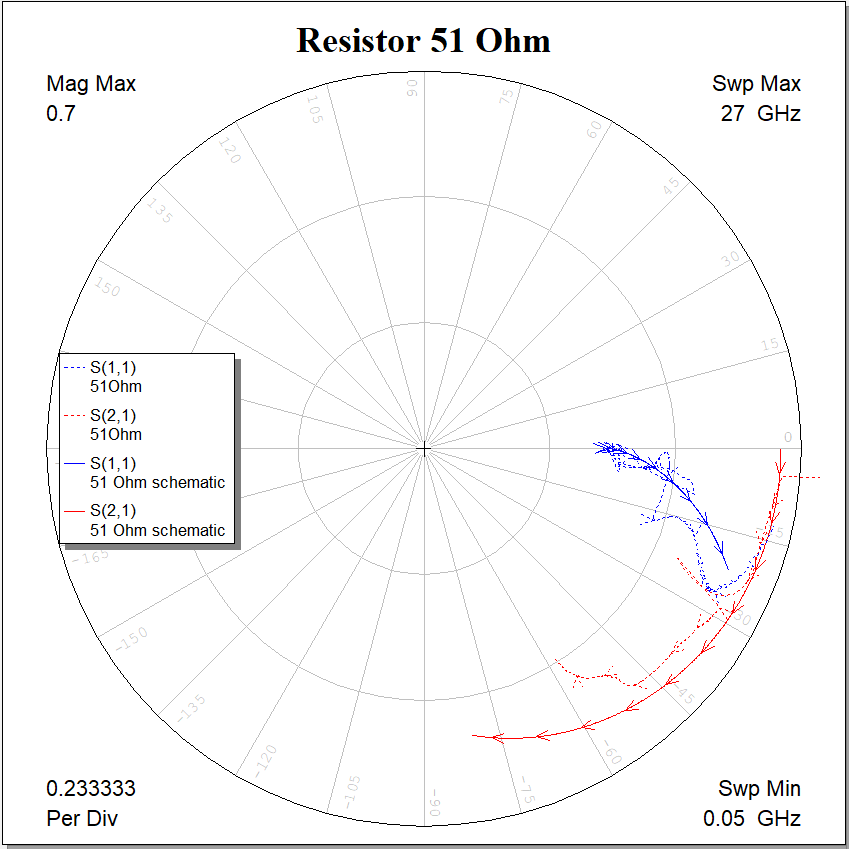
\includegraphics[width=\textwidth]{src/resistor-51Ohm.png}
    \caption{\label{fig:resistor-51Ohm}$51\Ohm$ rezistor}
\end{subfigure}\\[3mm]
\begin{subfigure}{0.45\textwidth}
    \centering
    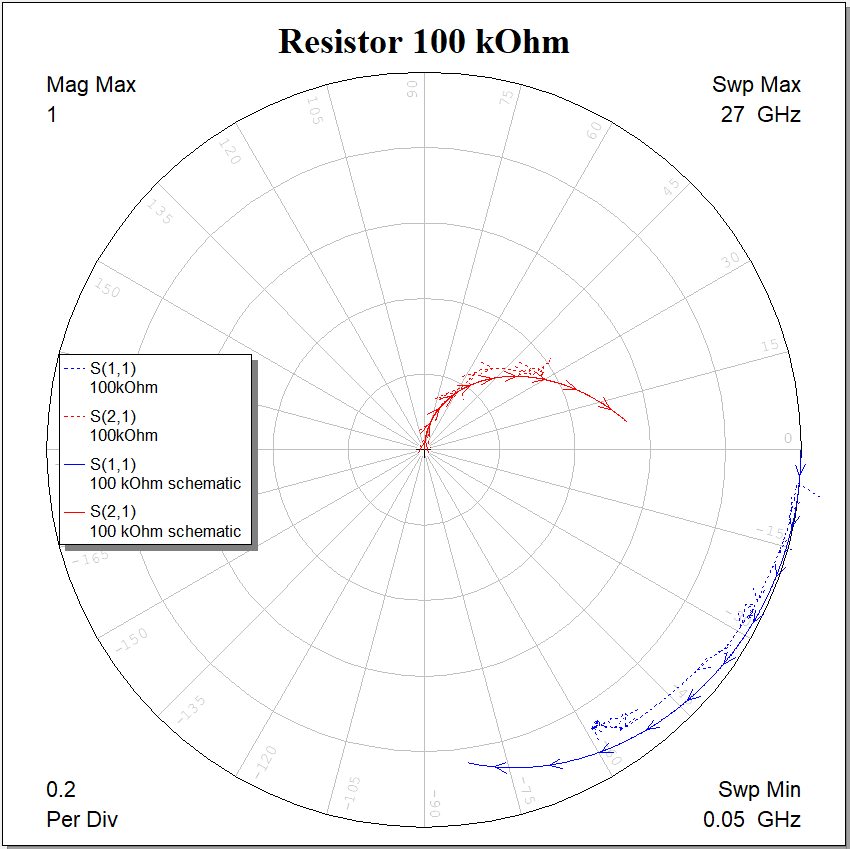
\includegraphics[width=\textwidth]{src/resistor-100kOhm.png}
    \caption{\label{fig:resistor-100kOhm}$100\kOhm$ rezistor}
\end{subfigure}
\caption{\label{fig:resistors}Porovnání naměřených S-parametrů rezistorů s daty dodanými výrobcem}
\end{figure}
\begin{table}[!ht]
    \centering
    \begin{tabular}{|c|c|c|}
        \hline
        $C_p\ [\mathrm{pF}]$ & $C_s\ [\mathrm{pF}]$ & $L_s\ [\mathrm{nH}]$\\
        \hline\hline
        0.054 & 0.027 & 0.38\\
        \hline
    \end{tabular}
    \caption{\label{table:parametry-pouzdra}Přibližné hodnoty parametrů pouzdra 0402}
\end{table}

\subsection*{Závěr}
V rámci laboratorní úlohy jsme se naučili využívat vektorového měření pro určování parametrů SMD komponent s referenční rovinou přímo na okrajích pouzdra. Mohli jsme tak pozorovat soulad takto naměřených S-parametrů s daty dodanými výrobcem a kvalitativně popsat i jejich nesrovnalosti.

Prvním úkolem bylo měření dvou $10\mathrm{pF}$ kondenzátorů od společností ATC a Johanson Technology, kde jsme naměřili velice uspokojivé výsledky až na vzájemný fázový posun dat. Měli jsme tak možnost se seznámit s velice běžnou praktikou výrobců, a to s tím, že dodávají S-parametry naměřené uprostřed pouzdra, což může při neopatrném návrhu způsobovat značné problémy.

Druhá úloha byla obdobného charakteru. Předmětem měření byly induktory od společnosti Johanson Technology s hodnotami $3.3\ \mathrm{nH}$ a $27\ \mathrm{nH}$. Zatímco první z těchto induktorů opět vykazoval dobrou souhlasnost s daty od výrobce, frekvenční průběh S-parametrů druhého induktoru se již lišil více. Jelikož druhá měřící skupina se s tímto problémem nesetkala, jedná se nejspíše o chybu měření.

Třetí úloha spočívala ve využítí tří měření s různými rezistory ($2.2\ \Ohm$, $51\ \Ohm$ a $100\ \kOhm$) ve stejném pouzdru (0402) za účelem určení elektrických parametrů tohoto pouzdra. Měření i následné zpracování proběhlo bez větších potíží.

\end{document}
